\section{Methodology}
The objective of the project is to produce a parameterized simulation 
that could represent an ad-hoc networking scenario and compare the effects 
of different parameters on the overall communications system in terms of 
per-user average success rate (succssfully received messages) 
and latency of those messages.

The simulation is developed in several compontents.
The first stage of the simulation is the map creation layer,
which places N users (ceullar devices) randomly on an \textit{n x m} map at a
given (x, y) coordinate with a given starting radius (communication range).
The map creation stage can be instaniated for a new simulation dynamically, 
but additional methods exist to process files containing generated lists of 
users so that statically determined arrangements can be tried.
This layer is leveraged to create several static lists of different quantity
and arrangements of users, which were used for analysis by the main simulation.
As an example, Figure \ref{fig:usergraph} is the userlist
generated for the Intensity Ratio simulation.
Each user is modeled as a black point with the radius of the user colored in
for visualization purposes.
\par
\begin{figure}
    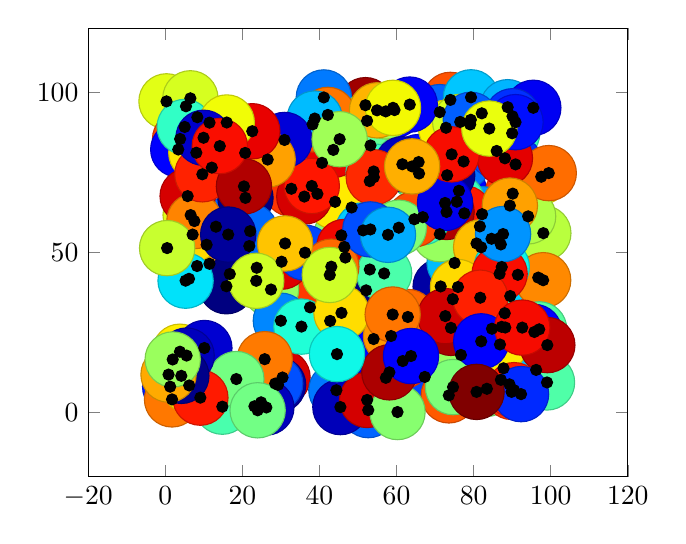
\begin{tikzpicture}

\begin{axis}[
xmin=-20, xmax=120,
ymin=-20, ymax=120,
axis on top
]
\addplot [only marks, scatter, scatter src=explicit, colormap={mymap}{[1pt]
  rgb(0pt)=(0,0,0.5);
  rgb(22pt)=(0,0,1);
  rgb(25pt)=(0,0,1);
  rgb(68pt)=(0,0.86,1);
  rgb(70pt)=(0,0.9,0.967741935483871);
  rgb(75pt)=(0.0806451612903226,1,0.887096774193548);
  rgb(128pt)=(0.935483870967742,1,0.0322580645161291);
  rgb(130pt)=(0.967741935483871,0.962962962962963,0);
  rgb(132pt)=(1,0.925925925925926,0);
  rgb(178pt)=(1,0.0740740740740741,0);
  rgb(182pt)=(0.909090909090909,0,0);
  rgb(200pt)=(0.5,0,0)
}, visualization depends on={\thisrow{sizedata} \as\perpointmarksize}, scatter/@pre marker code/.append style={/tikz/mark size=\perpointmarksize}]
table [x=x, y=y, meta=colordata]{%
x                      y                      colordata              sizedata
+7.459090885475142e+01 +3.539363377257585e+01 +6.685972099374399e-01 +1.000000000000000e+01
+1.072648067505945e+01 +5.237244617103784e+01 +4.798708121888173e-01 +1.000000000000000e+01
+8.161773952416821e+01 +5.811300790300644e+01 +9.894231117543170e-01 +1.000000000000000e+01
+4.834642700136421e+01 +6.401694267132378e+01 +6.211283300248572e-01 +1.000000000000000e+01
+3.041703763376190e+01 +1.092274426183900e+01 +9.214874440034894e-01 +1.000000000000000e+01
+7.617824939843777e+01 +6.924233949153952e+01 +1.337328331873407e-01 +1.000000000000000e+01
+9.012886591473981e+01 +6.834498110644745e+01 +8.505563247814649e-01 +1.000000000000000e+01
+8.999104673474069e+01 +8.719790096499403e+01 +4.180496935856070e-01 +1.000000000000000e+01
+8.949398064943543e+01 +3.635965505268689e+01 +7.732075734705480e-01 +1.000000000000000e+01
+4.065976584323990e+01 +7.795946195634635e+01 +3.407799557079070e-01 +1.000000000000000e+01
+9.753884440914430e+01 +7.361404255698994e+01 +6.574373013172986e-01 +1.000000000000000e+01
+6.732501674366254e+01 +1.110486244064456e+01 +1.994302411137353e-01 +1.000000000000000e+01
+1.314642908238736e+01 +5.802145335656703e+01 +2.235071593508359e-01 +1.000000000000000e+01
+8.704854841302708e+01 +5.247791773154085e+01 +9.172226335719869e-01 +1.000000000000000e+01
+8.210817375353699e+01 +9.342638177214066e+01 +3.317317140430129e-01 +1.000000000000000e+01
+7.670284874322209e+01 +1.797700651606122e+01 +5.358358895257488e-01 +1.000000000000000e+01
+2.072271754474474e+01 +8.105274892401192e+01 +8.626795882320477e-01 +1.000000000000000e+01
+4.438832846192208e+01 +6.948757327248122e+00 +2.500728020268650e-01 +1.000000000000000e+01
+7.739869754512634e+01 +7.838456490779974e+01 +2.398797424719341e-01 +1.000000000000000e+01
+3.270208738980129e+01 +6.986992094648002e+01 +8.512910807842052e-01 +1.000000000000000e+01
+4.567192881369905e+01 +5.531416843518837e+01 +5.113789572854077e-01 +1.000000000000000e+01
+8.074745798907432e+01 +5.278625726470998e+01 +6.441595651789217e-01 +1.000000000000000e+01
+3.800618539388456e+00 +1.898035223689788e+01 +6.604176079905619e-01 +1.000000000000000e+01
+7.144504813871809e+01 +3.936059813620913e+01 +4.218089127301572e-02 +1.000000000000000e+01
+7.396305897822700e+01 +9.761773054583462e+01 +8.212757902525076e-01 +1.000000000000000e+01
+1.270745159588615e+00 +8.064273835847224e+00 +1.627730396316432e-01 +1.000000000000000e+01
+5.323942877143768e+01 +8.340942724332746e+01 +8.031682534481044e-01 +1.000000000000000e+01
+5.369519592670735e+00 +9.562250006345330e+01 +3.870562688904696e-01 +1.000000000000000e+01
+6.154942288244847e+00 +4.173772357829102e+01 +3.867480725967365e-01 +1.000000000000000e+01
+2.925862978550109e+01 +8.631139407524968e+00 +3.574697539310046e-02 +1.000000000000000e+01
+4.277546513846524e+01 +2.860549030064020e+01 +8.095548818098083e-01 +1.000000000000000e+01
+8.322064202194335e+00 +9.220460155446591e+01 +7.914664934647173e-01 +1.000000000000000e+01
+3.165110489601886e-01 +9.715469482611766e+01 +6.257334922635519e-01 +1.000000000000000e+01
+8.463542898004346e+01 +5.424664799258552e+01 +7.962576334985538e-01 +1.000000000000000e+01
+8.641161769611119e+01 +5.426984704255544e+01 +2.286758026089172e-01 +1.000000000000000e+01
+7.355960263914938e+01 +5.349449932574424e+00 +8.132289090472478e-01 +1.000000000000000e+01
+3.754349772773659e+01 +3.282987029320351e+01 +8.458128884613919e-01 +1.000000000000000e+01
+8.218839925749361e+01 +6.192201382490909e+01 +2.760313997110988e-01 +1.000000000000000e+01
+9.675551069151030e+01 +4.212176738330419e+01 +8.410548731824899e-01 +1.000000000000000e+01
+7.505700353425038e+01 +4.668878136878691e+01 +3.154108016442078e-01 +1.000000000000000e+01
+2.312851447393848e+01 +1.936697515232211e+00 +2.173168027510437e-01 +1.000000000000000e+01
+3.945900937818263e+01 +6.826783483491251e+01 +9.584295100679692e-01 +1.000000000000000e+01
+1.673493876093390e+01 +4.324763883254897e+01 +3.101009581936455e-01 +1.000000000000000e+01
+2.484921902521985e+01 +3.169244833562890e+00 +5.452520123644984e-01 +1.000000000000000e+01
+5.266031635086029e+01 +7.467706390247297e-01 +2.297972258037179e-01 +1.000000000000000e+01
+5.304950811926778e+01 +7.224329498163958e+01 +5.446527235829153e-01 +1.000000000000000e+01
+8.929980915371722e+01 +8.789321664683559e+00 +8.441868110605634e-01 +1.000000000000000e+01
+7.563682390342728e+01 +6.581221798257452e+01 +4.210215015850803e-01 +1.000000000000000e+01
+1.146611946203677e+01 +4.643457777953001e+01 +8.636523092442028e-02 +1.000000000000000e+01
+2.743089153111639e+01 +3.839822922061242e+01 +5.337316153826164e-01 +1.000000000000000e+01
+8.725352438752533e+01 +2.675140892080330e+01 +4.275369973164085e-01 +1.000000000000000e+01
+4.405513398491767e+01 +6.578958091732331e+01 +6.619255016842206e-01 +1.000000000000000e+01
+6.583333031850593e+01 +7.461827951728662e+01 +4.794425107689720e-01 +1.000000000000000e+01
+2.372919261408384e+01 +4.519539307027510e+01 +5.929295410813413e-01 +1.000000000000000e+01
+7.410524436539805e+01 +2.643559619931185e+01 +9.627510018914293e-01 +1.000000000000000e+01
+9.146740937151144e+01 +4.299121238568523e+01 +5.782115356514119e-01 +1.000000000000000e+01
+5.947504429580608e+01 +9.443330922410807e+01 +1.235531648520408e-01 +1.000000000000000e+01
+5.305727994754640e+01 +4.465193766982800e+01 +1.609855768953745e-01 +1.000000000000000e+01
+5.404708137176709e+01 +2.293863872516334e+01 +1.139336505899891e-01 +1.000000000000000e+01
+4.671790404488846e+01 +4.838217686859174e+01 +4.028339377767198e-01 +1.000000000000000e+01
+2.851040682705223e+01 +9.034387583693015e+00 +2.104545974149497e-01 +1.000000000000000e+01
+5.722735040371067e+01 +1.082493903566848e+01 +9.955627860928884e-02 +1.000000000000000e+01
+4.543014200135944e+01 +1.695251059673819e+00 +5.888674987930420e-02 +1.000000000000000e+01
+9.807802509001029e+01 +5.600129103980949e+01 +5.761322152541913e-01 +1.000000000000000e+01
+8.475443772738603e+01 +2.615189019686553e+01 +3.580225122271710e-01 +1.000000000000000e+01
+3.017124029929794e+01 +4.709554240159954e+01 +9.147046294050275e-01 +1.000000000000000e+01
+2.621702174056087e+01 +1.567848107048908e+00 +6.164119060230921e-02 +1.000000000000000e+01
+4.359374117789365e+01 +8.200136933690175e+01 +9.058930222165679e-01 +1.000000000000000e+01
+6.572393857596504e+01 +7.820232085537589e+01 +1.403173964240205e-01 +1.000000000000000e+01
+5.192478638224611e+01 +9.596383682377268e+01 +9.680196696341239e-01 +1.000000000000000e+01
+5.236715061434669e+01 +3.920698196548478e+00 +9.236885691755949e-01 +1.000000000000000e+01
+7.910864281359142e+01 +8.994298977131629e+01 +6.267198250802942e-01 +1.000000000000000e+01
+1.147594637069317e+01 +9.051196875737256e+01 +5.783738442802011e-02 +1.000000000000000e+01
+8.706428765939478e+01 +1.018942668320667e+01 +1.114640278386124e-01 +1.000000000000000e+01
+6.160399494587533e+01 +1.606274672321383e+01 +8.421725099541121e-01 +1.000000000000000e+01
+7.757862640126535e+01 +6.219042588378608e+01 +8.804647624110871e-01 +1.000000000000000e+01
+7.122239393396418e+01 +5.569186345110288e+01 +5.365746558812284e-01 +1.000000000000000e+01
+7.120480081123996e+01 +9.379031381566595e+01 +2.292640646274660e-01 +1.000000000000000e+01
+6.293019415932374e+01 +2.983060374008699e+01 +7.956504453663424e-01 +1.000000000000000e+01
+2.998523233361318e+01 +2.865829251379111e+01 +2.637637706927377e-01 +1.000000000000000e+01
+3.850797995356847e+00 +8.540249755455901e+01 +8.350662315789855e-01 +1.000000000000000e+01
+8.807041540308487e+01 +3.099466392423209e+01 +3.383670948355719e-01 +1.000000000000000e+01
+4.113458612992207e+01 +9.837920673438860e+01 +2.508378030228012e-01 +1.000000000000000e+01
+3.821317148673150e+01 +8.996973752017681e+01 +8.213397599576071e-01 +1.000000000000000e+01
+7.313126289823762e+01 +7.408564282688064e+01 +2.639189487163796e-02 +1.000000000000000e+01
+7.283550013914660e+01 +8.890778335052207e+01 +6.527369954459536e-01 +1.000000000000000e+01
+7.931672011485927e+01 +9.841701545234723e+01 +3.247014679427226e-01 +1.000000000000000e+01
+5.235605347755700e+01 +9.108157960686437e+01 +4.700473327200674e-01 +1.000000000000000e+01
+5.407026653313798e+01 +7.526527973514798e+01 +4.213079664983114e-01 +1.000000000000000e+01
+9.803387610929305e+01 +4.130870467770843e+01 +7.639318207144506e-01 +1.000000000000000e+01
+4.217361741599767e+01 +9.293018593422953e+01 +7.837963705702670e-01 +1.000000000000000e+01
+5.210408192291168e+01 +3.814445159320468e+01 +1.200906618991215e-02 +1.000000000000000e+01
+8.882507720276091e+01 +9.533107892178081e+01 +3.078626306377292e-01 +1.000000000000000e+01
+2.079852278170107e+01 +6.701840212898479e+01 +1.263669190665240e-02 +1.000000000000000e+01
+7.297217619390560e+01 +6.262187052058514e+01 +9.561095813733824e-01 +1.000000000000000e+01
+5.720143427537271e+01 +9.402771890407749e+01 +5.472442282245766e-01 +1.000000000000000e+01
+5.132874215707817e+01 +5.686399849163885e+01 +3.300918422700292e-01 +1.000000000000000e+01
+6.580967905112645e+00 +6.163901125309989e+01 +6.242987962383173e-01 +1.000000000000000e+01
+9.547861210614357e+01 +9.514816629597819e+01 +1.085981437008798e-01 +1.000000000000000e+01
+1.013941140793581e+01 +2.013007168213992e+01 +7.973885510480649e-02 +1.000000000000000e+01
+9.087173426163231e+01 +7.747494801953870e+01 +1.806235279930180e-01 +1.000000000000000e+01
+3.607020624746586e+01 +6.742828269067657e+01 +9.220824541851672e-01 +1.000000000000000e+01
+9.622086587153277e+01 +1.329716244839011e+01 +2.599335476423219e-01 +1.000000000000000e+01
+6.024308324255655e+01 +1.435611791790303e-01 +5.172643335021938e-01 +1.000000000000000e+01
+8.820247352368149e+01 +2.654774822820783e+01 +4.380890298843174e-01 +1.000000000000000e+01
+2.179729430287628e+01 +5.197513410910555e+01 +6.162758402429764e-01 +1.000000000000000e+01
+3.623944240079797e+01 +4.990849473077168e+01 +2.006003826239193e-01 +1.000000000000000e+01
+1.480660247942894e+01 +1.816978609272435e+00 +4.428876563458933e-01 +1.000000000000000e+01
+1.206977036880065e+01 +7.647107385375442e+01 +6.234075001736420e-01 +1.000000000000000e+01
+5.493604582867830e+01 +9.436068177113258e+01 +7.193805852029853e-01 +1.000000000000000e+01
+8.194373134482559e+01 +5.160380973485592e+01 +7.077866564219958e-01 +1.000000000000000e+01
+5.857156735388570e+01 +2.388008236875597e+01 +7.496292547790101e-01 +1.000000000000000e+01
+3.368610024537699e+00 +8.212779495941214e+01 +1.302357288187436e-01 +1.000000000000000e+01
+8.597122508592413e+01 +8.166881367116143e+01 +1.980779138469522e-01 +1.000000000000000e+01
+1.758362923667312e+00 +4.092634815771879e+00 +7.813507959486232e-01 +1.000000000000000e+01
+6.512012000911582e+00 +9.810779124586388e+01 +6.117663229987776e-01 +1.000000000000000e+01
+4.645785838628610e+01 +5.169063222318141e+01 +8.998646450168740e-01 +1.000000000000000e+01
+6.681674901065038e+01 +6.099918009688587e+01 +4.186696870746108e-01 +1.000000000000000e+01
+7.465087030491385e+01 +7.932409145719599e+00 +5.061891723737593e-01 +1.000000000000000e+01
+9.700087359325920e+01 +2.596560474758053e+01 +4.597580285919176e-01 +1.000000000000000e+01
+7.651450673648564e+01 +9.073877650750524e+01 +6.128294440702259e-01 +1.000000000000000e+01
+6.150684566139567e+01 +7.752006783105070e+01 +6.417400437724174e-02 +1.000000000000000e+01
+9.574653849043506e+01 +2.514891011559138e+01 +1.264657519800743e-01 +1.000000000000000e+01
+6.342030703072656e+01 +9.614930369344094e+01 +1.135827957496407e-01 +1.000000000000000e+01
+5.409521760509549e+01 +7.345915449354668e+01 +8.641681518881147e-01 +1.000000000000000e+01
+2.201502491643398e+01 +5.663637637343355e+01 +2.361089532754828e-01 +1.000000000000000e+01
+6.462544767124983e+01 +6.035172305602583e+01 +8.270161343389343e-01 +1.000000000000000e+01
+6.057394999248588e+01 +5.771315412685237e+01 +5.106595128554677e-01 +1.000000000000000e+01
+3.800671304989471e+01 +7.073222919902936e+01 +8.838906167432402e-01 +1.000000000000000e+01
+3.532384749547237e+01 +2.682157853671909e+01 +3.936040925672729e-01 +1.000000000000000e+01
+2.579528734708152e+01 +1.664593511575584e+01 +7.792522632204935e-01 +1.000000000000000e+01
+5.677303402642558e+01 +4.342031719556114e+01 +4.453110650811438e-01 +1.000000000000000e+01
+3.877222039204145e+01 +9.179064525500809e+01 +3.147546483679468e-01 +1.000000000000000e+01
+8.250878824658326e+00 +4.573931516784695e+01 +7.492618749381471e-01 +1.000000000000000e+01
+3.093334054917970e+01 +8.510563371849264e+01 +8.565516954093311e-02 +1.000000000000000e+01
+6.204134960601026e+00 +8.443678155981772e+00 +6.704596865983899e-01 +1.000000000000000e+01
+9.413291996700042e+01 +6.124392104814707e+01 +5.664205306416742e-01 +1.000000000000000e+01
+7.593783478564514e+01 +3.918502017295950e+01 +6.790374263220605e-01 +1.000000000000000e+01
+8.729041750632331e+01 +4.542964305575401e+01 +3.706236391101343e-01 +1.000000000000000e+01
+1.842992677394889e+01 +1.043855648028923e+01 +4.945304793212525e-01 +1.000000000000000e+01
+5.804018191269322e+00 +6.756909986000295e+01 +9.218524680670850e-01 +1.000000000000000e+01
+7.092916489228340e+00 +5.556387033054001e+01 +6.815192482661730e-01 +1.000000000000000e+01
+8.343670212323575e+01 +7.404081768954674e+00 +5.044840867385008e-01 +1.000000000000000e+01
+8.052605223181974e+00 +8.111936689380890e+01 +6.638430815842630e-01 +1.000000000000000e+01
+9.903196202886345e+01 +9.384277356699133e+00 +4.491356082430378e-01 +1.000000000000000e+01
+4.570896590965635e+01 +3.109820218046596e+01 +6.765067033554027e-01 +1.000000000000000e+01
+7.557347650672563e+00 +5.977402431324604e+01 +7.695034070647101e-01 +1.000000000000000e+01
+2.656523306030011e+01 +7.898703959378834e+01 +7.392656110961309e-01 +1.000000000000000e+01
+1.586108914749978e+01 +3.942383948650046e+01 +1.033132749310683e-02 +1.000000000000000e+01
+9.100421940518732e+00 +4.635066545441613e+00 +8.800230538533926e-01 +1.000000000000000e+01
+4.307778170653441e+01 +4.553510250670586e+01 +7.975168762826715e-01 +1.000000000000000e+01
+9.616757863274227e+00 +7.438334919531330e+01 +8.709965592396278e-01 +1.000000000000000e+01
+7.265029562224775e+01 +3.010222907810620e+01 +9.258682720613137e-01 +1.000000000000000e+01
+3.107902504294012e+01 +5.279017687955212e+01 +7.023177651487452e-01 +1.000000000000000e+01
+2.040759226958603e+01 +7.060418579654349e+01 +9.529551107368488e-01 +1.000000000000000e+01
+5.814055326779213e+01 +1.253839615303524e+01 +9.572460296334709e-01 +1.000000000000000e+01
+4.454830642657104e+01 +1.822858638810698e+01 +3.729868210704262e-01 +1.000000000000000e+01
+9.948502117499852e+01 +7.475415199645964e+01 +7.929603196890149e-01 +1.000000000000000e+01
+8.673077086992922e+01 +4.329770140687202e+01 +8.917112746768528e-01 +1.000000000000000e+01
+8.775387904153543e+01 +1.380086672235901e+01 +3.114902836742900e-01 +1.000000000000000e+01
+8.984700579326464e+01 +6.438286754531108e+00 +8.549911197952380e-01 +1.000000000000000e+01
+5.532533044673393e+00 +1.777310091533960e+01 +6.072193316804175e-02 +1.000000000000000e+01
+8.171733421029397e+01 +3.584383088794102e+01 +8.737265753604265e-01 +1.000000000000000e+01
+8.682959759457482e+01 +2.123810467323237e+01 +6.592846187065085e-01 +1.000000000000000e+01
+5.268689399960113e+00 +4.116361352120831e+01 +3.516579354073125e-01 +1.000000000000000e+01
+4.159995370151570e+00 +1.144543132648426e+01 +1.821602378381981e-02 +1.000000000000000e+01
+5.033331370698413e+00 +8.916768128607931e+01 +4.134056001790173e-01 +1.000000000000000e+01
+5.899859289397153e+01 +3.059842113141757e+01 +7.839876265170730e-01 +1.000000000000000e+01
+9.008444498607780e+01 +9.250443027384546e+01 +1.799103969178105e-01 +1.000000000000000e+01
+9.046730765018492e+01 +6.968994991742560e+00 +8.753460589971135e-01 +1.000000000000000e+01
+1.632482971974070e+01 +5.556714820699867e+01 +3.387011538455076e-02 +1.000000000000000e+01
+8.455008741931502e-01 +1.183457444290238e+01 +7.294583250979670e-01 +1.000000000000000e+01
+7.926347696687712e+01 +9.140659748396513e+01 +2.250185952900868e-01 +1.000000000000000e+01
+2.359856258219952e+01 +4.112296877537342e+01 +6.040529698473094e-01 +1.000000000000000e+01
+8.811046366838360e+01 +7.937988770321795e+01 +9.100780728038351e-01 +1.000000000000000e+01
+7.258474561124527e+01 +6.542779314499903e+01 +1.036796636131921e-01 +1.000000000000000e+01
+7.429130625742468e+01 +8.061045537541304e+01 +8.933898590395862e-01 +1.000000000000000e+01
+4.523545806435965e+01 +8.534581250989082e+01 +5.465169346624772e-01 +1.000000000000000e+01
+2.396338327293702e+01 +6.894188462779893e-01 +4.914183212635037e-01 +1.000000000000000e+01
+8.196391685459649e+01 +2.221859407287259e+01 +1.255413114866409e-01 +1.000000000000000e+01
+5.320527127049185e+01 +5.716683613610348e+01 +2.086457421951077e-01 +1.000000000000000e+01
+4.815062689649929e-01 +5.133946237659998e+01 +5.943992970411992e-01 +1.000000000000000e+01
+2.256905766152508e+01 +8.782609968240450e+01 +9.053047896169728e-01 +1.000000000000000e+01
+9.911060649170091e+01 +2.104633898344873e+01 +9.440873975988913e-01 +1.000000000000000e+01
+1.595062711896409e+01 +9.056337611127668e+01 +6.432818815086049e-01 +1.000000000000000e+01
+9.086129772473225e+01 +9.066743843847992e+01 +1.476861226100923e-01 +1.000000000000000e+01
+5.777840340781819e+01 +5.548631158641657e+01 +2.994361172685142e-01 +1.000000000000000e+01
+9.229699977516601e+01 +5.738491987060179e+00 +1.730921128418241e-01 +1.000000000000000e+01
+8.939633262456015e+01 +6.461282587925416e+01 +7.389211628534655e-01 +1.000000000000000e+01
+8.075130019463877e+01 +6.432771209983235e+00 +9.954088947494172e-01 +1.000000000000000e+01
+6.374408786673652e+01 +1.762680989371956e+01 +1.239578942034140e-01 +1.000000000000000e+01
+9.925999863109524e+00 +8.579115248996982e+01 +7.465778033341131e-02 +1.000000000000000e+01
+9.260849192584708e+01 +2.650805439570959e+01 +8.949415896662594e-01 +1.000000000000000e+01
+8.405900549379132e+01 +8.866754648374462e+01 +6.350461040407924e-01 +1.000000000000000e+01
+6.403396481426142e+01 +7.685340872643881e+01 +7.240477422232607e-01 +1.000000000000000e+01
+1.922027135695925e+00 +1.655474457729900e+01 +5.395570522007921e-01 +1.000000000000000e+01
+1.414336199854279e+01 +8.319151262311733e+01 +8.916793049978626e-01 +1.000000000000000e+01
+8.763140763247125e+01 +5.572020039780769e+01 +2.766960524550772e-01 +1.000000000000000e+01
+4.267724611056355e+01 +4.294845060565535e+01 +6.024288095637429e-01 +1.000000000000000e+01
+5.908274588538549e+01 +9.513757133627234e+01 +6.466389113334630e-01 +1.000000000000000e+01
};
\addplot [only marks, draw=black, fill=black, colormap={mymap}{[1pt]
  rgb(0pt)=(0,0,0.5);
  rgb(22pt)=(0,0,1);
  rgb(25pt)=(0,0,1);
  rgb(68pt)=(0,0.86,1);
  rgb(70pt)=(0,0.9,0.967741935483871);
  rgb(75pt)=(0.0806451612903226,1,0.887096774193548);
  rgb(128pt)=(0.935483870967742,1,0.0322580645161291);
  rgb(130pt)=(0.967741935483871,0.962962962962963,0);
  rgb(132pt)=(1,0.925925925925926,0);
  rgb(178pt)=(1,0.0740740740740741,0);
  rgb(182pt)=(0.909090909090909,0,0);
  rgb(200pt)=(0.5,0,0)
}]
table {%
x                      y
+7.459090885475142e+01 +3.539363377257585e+01
+1.072648067505945e+01 +5.237244617103784e+01
+8.161773952416821e+01 +5.811300790300644e+01
+4.834642700136421e+01 +6.401694267132378e+01
+3.041703763376190e+01 +1.092274426183900e+01
+7.617824939843777e+01 +6.924233949153952e+01
+9.012886591473981e+01 +6.834498110644745e+01
+8.999104673474069e+01 +8.719790096499403e+01
+8.949398064943543e+01 +3.635965505268689e+01
+4.065976584323990e+01 +7.795946195634635e+01
+9.753884440914430e+01 +7.361404255698994e+01
+6.732501674366254e+01 +1.110486244064456e+01
+1.314642908238736e+01 +5.802145335656703e+01
+8.704854841302708e+01 +5.247791773154085e+01
+8.210817375353699e+01 +9.342638177214066e+01
+7.670284874322209e+01 +1.797700651606122e+01
+2.072271754474474e+01 +8.105274892401192e+01
+4.438832846192208e+01 +6.948757327248122e+00
+7.739869754512634e+01 +7.838456490779974e+01
+3.270208738980129e+01 +6.986992094648002e+01
+4.567192881369905e+01 +5.531416843518837e+01
+8.074745798907432e+01 +5.278625726470998e+01
+3.800618539388456e+00 +1.898035223689788e+01
+7.144504813871809e+01 +3.936059813620913e+01
+7.396305897822700e+01 +9.761773054583462e+01
+1.270745159588615e+00 +8.064273835847224e+00
+5.323942877143768e+01 +8.340942724332746e+01
+5.369519592670735e+00 +9.562250006345330e+01
+6.154942288244847e+00 +4.173772357829102e+01
+2.925862978550109e+01 +8.631139407524968e+00
+4.277546513846524e+01 +2.860549030064020e+01
+8.322064202194335e+00 +9.220460155446591e+01
+3.165110489601886e-01 +9.715469482611766e+01
+8.463542898004346e+01 +5.424664799258552e+01
+8.641161769611119e+01 +5.426984704255544e+01
+7.355960263914938e+01 +5.349449932574424e+00
+3.754349772773659e+01 +3.282987029320351e+01
+8.218839925749361e+01 +6.192201382490909e+01
+9.675551069151030e+01 +4.212176738330419e+01
+7.505700353425038e+01 +4.668878136878691e+01
+2.312851447393848e+01 +1.936697515232211e+00
+3.945900937818263e+01 +6.826783483491251e+01
+1.673493876093390e+01 +4.324763883254897e+01
+2.484921902521985e+01 +3.169244833562890e+00
+5.266031635086029e+01 +7.467706390247297e-01
+5.304950811926778e+01 +7.224329498163958e+01
+8.929980915371722e+01 +8.789321664683559e+00
+7.563682390342728e+01 +6.581221798257452e+01
+1.146611946203677e+01 +4.643457777953001e+01
+2.743089153111639e+01 +3.839822922061242e+01
+8.725352438752533e+01 +2.675140892080330e+01
+4.405513398491767e+01 +6.578958091732331e+01
+6.583333031850593e+01 +7.461827951728662e+01
+2.372919261408384e+01 +4.519539307027510e+01
+7.410524436539805e+01 +2.643559619931185e+01
+9.146740937151144e+01 +4.299121238568523e+01
+5.947504429580608e+01 +9.443330922410807e+01
+5.305727994754640e+01 +4.465193766982800e+01
+5.404708137176709e+01 +2.293863872516334e+01
+4.671790404488846e+01 +4.838217686859174e+01
+2.851040682705223e+01 +9.034387583693015e+00
+5.722735040371067e+01 +1.082493903566848e+01
+4.543014200135944e+01 +1.695251059673819e+00
+9.807802509001029e+01 +5.600129103980949e+01
+8.475443772738603e+01 +2.615189019686553e+01
+3.017124029929794e+01 +4.709554240159954e+01
+2.621702174056087e+01 +1.567848107048908e+00
+4.359374117789365e+01 +8.200136933690175e+01
+6.572393857596504e+01 +7.820232085537589e+01
+5.192478638224611e+01 +9.596383682377268e+01
+5.236715061434669e+01 +3.920698196548478e+00
+7.910864281359142e+01 +8.994298977131629e+01
+1.147594637069317e+01 +9.051196875737256e+01
+8.706428765939478e+01 +1.018942668320667e+01
+6.160399494587533e+01 +1.606274672321383e+01
+7.757862640126535e+01 +6.219042588378608e+01
+7.122239393396418e+01 +5.569186345110288e+01
+7.120480081123996e+01 +9.379031381566595e+01
+6.293019415932374e+01 +2.983060374008699e+01
+2.998523233361318e+01 +2.865829251379111e+01
+3.850797995356847e+00 +8.540249755455901e+01
+8.807041540308487e+01 +3.099466392423209e+01
+4.113458612992207e+01 +9.837920673438860e+01
+3.821317148673150e+01 +8.996973752017681e+01
+7.313126289823762e+01 +7.408564282688064e+01
+7.283550013914660e+01 +8.890778335052207e+01
+7.931672011485927e+01 +9.841701545234723e+01
+5.235605347755700e+01 +9.108157960686437e+01
+5.407026653313798e+01 +7.526527973514798e+01
+9.803387610929305e+01 +4.130870467770843e+01
+4.217361741599767e+01 +9.293018593422953e+01
+5.210408192291168e+01 +3.814445159320468e+01
+8.882507720276091e+01 +9.533107892178081e+01
+2.079852278170107e+01 +6.701840212898479e+01
+7.297217619390560e+01 +6.262187052058514e+01
+5.720143427537271e+01 +9.402771890407749e+01
+5.132874215707817e+01 +5.686399849163885e+01
+6.580967905112645e+00 +6.163901125309989e+01
+9.547861210614357e+01 +9.514816629597819e+01
+1.013941140793581e+01 +2.013007168213992e+01
+9.087173426163231e+01 +7.747494801953870e+01
+3.607020624746586e+01 +6.742828269067657e+01
+9.622086587153277e+01 +1.329716244839011e+01
+6.024308324255655e+01 +1.435611791790303e-01
+8.820247352368149e+01 +2.654774822820783e+01
+2.179729430287628e+01 +5.197513410910555e+01
+3.623944240079797e+01 +4.990849473077168e+01
+1.480660247942894e+01 +1.816978609272435e+00
+1.206977036880065e+01 +7.647107385375442e+01
+5.493604582867830e+01 +9.436068177113258e+01
+8.194373134482559e+01 +5.160380973485592e+01
+5.857156735388570e+01 +2.388008236875597e+01
+3.368610024537699e+00 +8.212779495941214e+01
+8.597122508592413e+01 +8.166881367116143e+01
+1.758362923667312e+00 +4.092634815771879e+00
+6.512012000911582e+00 +9.810779124586388e+01
+4.645785838628610e+01 +5.169063222318141e+01
+6.681674901065038e+01 +6.099918009688587e+01
+7.465087030491385e+01 +7.932409145719599e+00
+9.700087359325920e+01 +2.596560474758053e+01
+7.651450673648564e+01 +9.073877650750524e+01
+6.150684566139567e+01 +7.752006783105070e+01
+9.574653849043506e+01 +2.514891011559138e+01
+6.342030703072656e+01 +9.614930369344094e+01
+5.409521760509549e+01 +7.345915449354668e+01
+2.201502491643398e+01 +5.663637637343355e+01
+6.462544767124983e+01 +6.035172305602583e+01
+6.057394999248588e+01 +5.771315412685237e+01
+3.800671304989471e+01 +7.073222919902936e+01
+3.532384749547237e+01 +2.682157853671909e+01
+2.579528734708152e+01 +1.664593511575584e+01
+5.677303402642558e+01 +4.342031719556114e+01
+3.877222039204145e+01 +9.179064525500809e+01
+8.250878824658326e+00 +4.573931516784695e+01
+3.093334054917970e+01 +8.510563371849264e+01
+6.204134960601026e+00 +8.443678155981772e+00
+9.413291996700042e+01 +6.124392104814707e+01
+7.593783478564514e+01 +3.918502017295950e+01
+8.729041750632331e+01 +4.542964305575401e+01
+1.842992677394889e+01 +1.043855648028923e+01
+5.804018191269322e+00 +6.756909986000295e+01
+7.092916489228340e+00 +5.556387033054001e+01
+8.343670212323575e+01 +7.404081768954674e+00
+8.052605223181974e+00 +8.111936689380890e+01
+9.903196202886345e+01 +9.384277356699133e+00
+4.570896590965635e+01 +3.109820218046596e+01
+7.557347650672563e+00 +5.977402431324604e+01
+2.656523306030011e+01 +7.898703959378834e+01
+1.586108914749978e+01 +3.942383948650046e+01
+9.100421940518732e+00 +4.635066545441613e+00
+4.307778170653441e+01 +4.553510250670586e+01
+9.616757863274227e+00 +7.438334919531330e+01
+7.265029562224775e+01 +3.010222907810620e+01
+3.107902504294012e+01 +5.279017687955212e+01
+2.040759226958603e+01 +7.060418579654349e+01
+5.814055326779213e+01 +1.253839615303524e+01
+4.454830642657104e+01 +1.822858638810698e+01
+9.948502117499852e+01 +7.475415199645964e+01
+8.673077086992922e+01 +4.329770140687202e+01
+8.775387904153543e+01 +1.380086672235901e+01
+8.984700579326464e+01 +6.438286754531108e+00
+5.532533044673393e+00 +1.777310091533960e+01
+8.171733421029397e+01 +3.584383088794102e+01
+8.682959759457482e+01 +2.123810467323237e+01
+5.268689399960113e+00 +4.116361352120831e+01
+4.159995370151570e+00 +1.144543132648426e+01
+5.033331370698413e+00 +8.916768128607931e+01
+5.899859289397153e+01 +3.059842113141757e+01
+9.008444498607780e+01 +9.250443027384546e+01
+9.046730765018492e+01 +6.968994991742560e+00
+1.632482971974070e+01 +5.556714820699867e+01
+8.455008741931502e-01 +1.183457444290238e+01
+7.926347696687712e+01 +9.140659748396513e+01
+2.359856258219952e+01 +4.112296877537342e+01
+8.811046366838360e+01 +7.937988770321795e+01
+7.258474561124527e+01 +6.542779314499903e+01
+7.429130625742468e+01 +8.061045537541304e+01
+4.523545806435965e+01 +8.534581250989082e+01
+2.396338327293702e+01 +6.894188462779893e-01
+8.196391685459649e+01 +2.221859407287259e+01
+5.320527127049185e+01 +5.716683613610348e+01
+4.815062689649929e-01 +5.133946237659998e+01
+2.256905766152508e+01 +8.782609968240450e+01
+9.911060649170091e+01 +2.104633898344873e+01
+1.595062711896409e+01 +9.056337611127668e+01
+9.086129772473225e+01 +9.066743843847992e+01
+5.777840340781819e+01 +5.548631158641657e+01
+9.229699977516601e+01 +5.738491987060179e+00
+8.939633262456015e+01 +6.461282587925416e+01
+8.075130019463877e+01 +6.432771209983235e+00
+6.374408786673652e+01 +1.762680989371956e+01
+9.925999863109524e+00 +8.579115248996982e+01
+9.260849192584708e+01 +2.650805439570959e+01
+8.405900549379132e+01 +8.866754648374462e+01
+6.403396481426142e+01 +7.685340872643881e+01
+1.922027135695925e+00 +1.655474457729900e+01
+1.414336199854279e+01 +8.319151262311733e+01
+8.763140763247125e+01 +5.572020039780769e+01
+4.267724611056355e+01 +4.294845060565535e+01
+5.908274588538549e+01 +9.513757133627234e+01
};
\end{axis}

\end{tikzpicture}

    \caption{User graph for 100 Users Randomly placed on a 100x100 grid}
    \label{fig:usergraph}
\end{figure}
\par

The second stage is the main simulation.
This stage took a list of users, as described previously, as well as additional
parameters describing the nature of communication amoung the users such as
the intensity ratio and the number of steps (as an analogue for time) to run 
the simulation for.
At each stage of the simulation, a randomly chosen subset of all users on the map
were chosen based upon the intensity ratio to attempt to send a message to another
randomly chosen user on the map.
After the number of steps specified is reached, the simulation would continue
to allow all users to complete their retransmission queues, which would usually
take a few extra steps to complete.
Once all users had finished their retransmissions, statistics would be compiled
on a per-user basis, and overall averages would be returned.

The main simulation stage is composed of several smaller elements modeling
the messages and user interactions.
These elements were modeled relatively simplisitically, so future additions could be
made to model other complex aspects of communication e.g. multi-packet messages,
fluctuating communication range, power usage, etc.

Finally, the last stage is a statistical analysis layer which enabled taking overall
statistics over a range of parameter values and creating relevant tables and graphs,
which are used in the results portion of this paper.

The language chosen to implement the simulation was Python, due to it's incorporation of 
object-oriented paradigms, as well as the ease of prototyping a larger program in a 
short period of time.
Additionally, the author's knowledge and existance of several data tools made it a natural
fit for this project.
A full listing of all the code created for this simulation is in Appendix \ref{appendix:code}.
